%!TEX encoding=UTF-8 Unicode
%!TEX root=../tabarnac.tex

\section{Expriments}
\label{sec:expe}
In this section, we show how to analyse and optimize NUMA memory behaviour using
\TABARNAC~ through two benchmarks. Finally we discuss our tool overhead.

\subsection{Setup}
\label{sec:expe-setup}

\begin{table}
    \centering
        \begin{tabular}{|l|c|c|c|c|c|}
            \hline
            \multirow{2}{*}{Global} & Nodes & Threads & Freq (GHz) & Memory (Gib) \\
            \cline{2-5}
                & $4$   & $64$ & $2.00$ & $124$ \\
            \hline
           \multirow{2}{*}{Per node} & Cores & Threads & L3 Cache (Mib) & Memory (GiB) \\
            \cline{2-5}
            & $8$ & $16$ & $18$Mib & $31$  \\
            \hline
        \end{tabular}
    \caption{Turing hardware}
    \label{tab:machines}
\end{table}

All the experiment were run on a NUMA machine composed of $4$ Intel Xeon X7550
processors, the hardware details are recapitulated in table \ref{tab:turing}.
The machine is running \texttt{Ubuntui 12.04.5 LTS} on a Linux kernel 3.13.0-48.
\DB{Other thing to mention, numctl version ?}

For the plots representing speedups, each configuration have been run 10 to 30
times and one point represent the mean of all runs.

\subsection{Analysis}
\label{sec:expe-analysis}

\subsubsection{Matrix multiplication}
\label{sec:exp-mat}

The first benchmark presented is based on a naive matrix multiplication
computing $C=A*B$. Our aim here is not to provide a kernel competing with the
state of the art, but to show how \TABARNAC~ can help to improve such
applications. We compare two implementations of the matrix multiplication, in
the first one, called \emph{Naive}, each threads start by computing
$C[0][tid]$ and then jumps $N$ elements after in the matrix, where $N$ is the
number of threads. Although this implementation is known to be bad, comparing
how much it's accelerated by the best mechanism to the acceleration of a
better version to understand the importance of the quality of the original
code. Moreover when an application have such a bad memory access pattern, it
is not always possible to change completely the pattern, therefore, it is
interesting to discuss the improvement we can obtain on this kernel without
modifying the algorithm. The second implementation uses a non recursive bloc
decomposition.

The figures presented in this sections are part of \TABARNAC~ visualization.
Each plot show for a particular data structure the number of memory accesses
per page and per threads. Only structures \texttt{B} and \texttt{C} are
presented as for both algorithm \texttt{A} have more are less the same access
pattern than \texttt{C}.

\begin{figure}[htb]
    \centering
    \subfigure[Structure B (naive)]{
        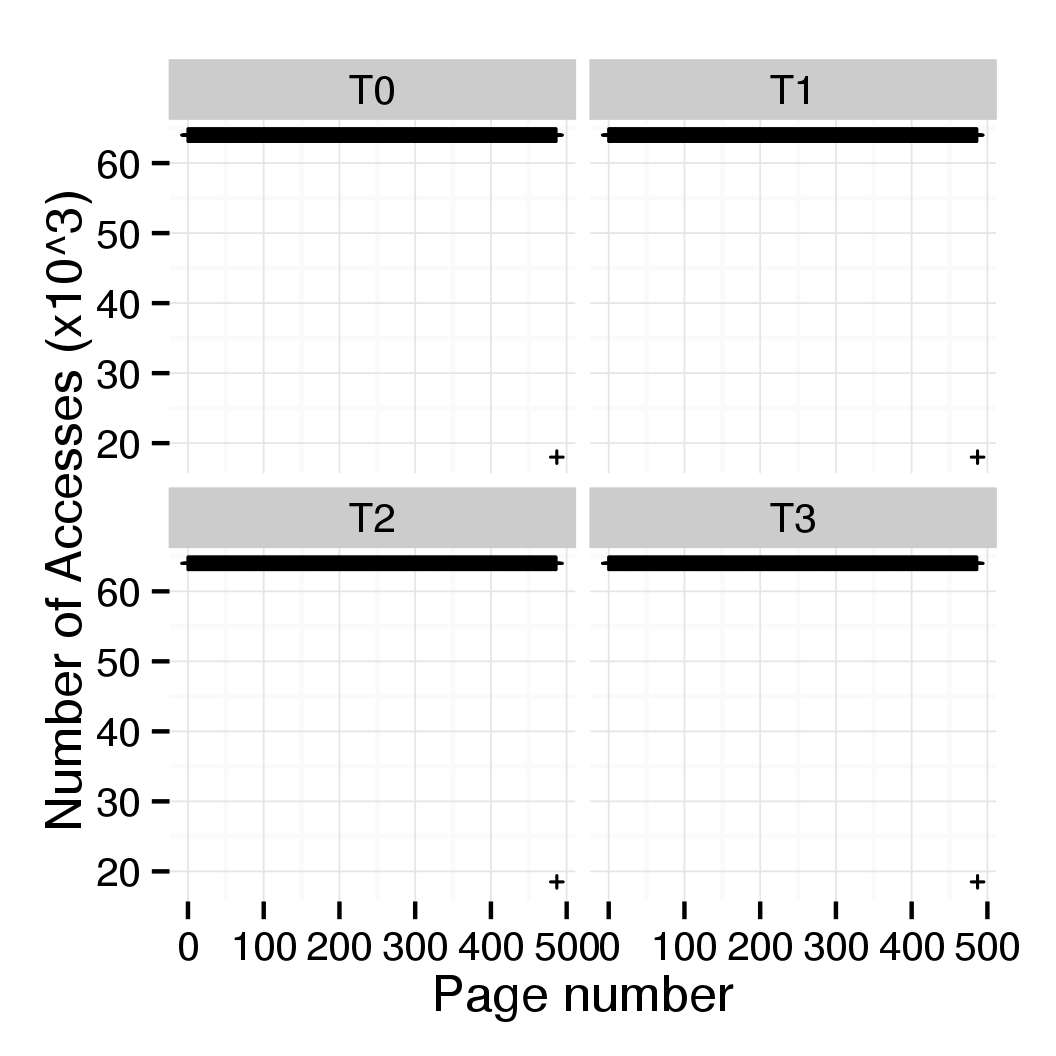
\includegraphics[height=.27\textheight] {mat_B_modulo}
        \label{fig:matrix-B-naive}
    }
    \subfigure[Structure C (naive)]{
        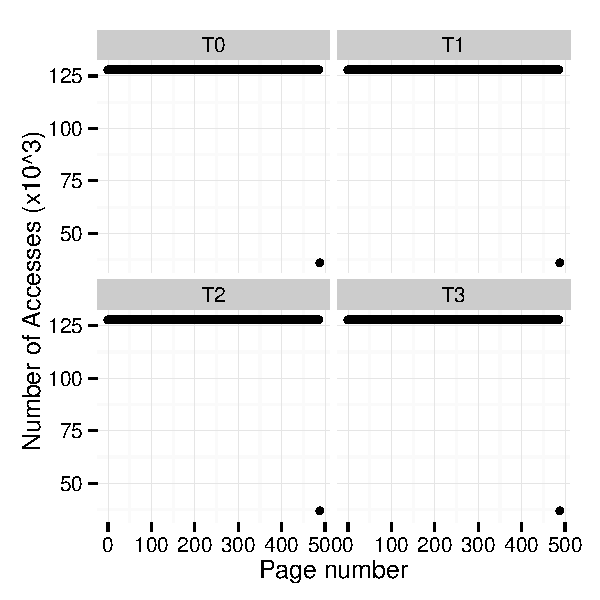
\includegraphics[height=.27\textheight] {mat_C_modulo}
        \label{fig:matrix-C-naive}
    }
    \caption{By thread access distribution on data structures A and B for the
        naive matrix multiplication. Each plots shows the number of access
    depending on the page number (inside the structure) for each thread.}
    \label{fig:matrix-naive}
\end{figure}

For the naive matrix multiplication, as we can see in
\ref{figure:matrix-naive}, all the pages of both structures are used by every
thread. Therefore, when we execute this code on a NUMA machine, wherever we
map the page, all the nodes but one will trigger remote memory accesses. We
can improve there are several ways to improve this behaviour: an easy solution
is to tell the operating system to interleave pages through the different
nodes. This will result on a better balance of memory bandwidth between the
nodes. An other solution is to create local copies of \texttt{A} and
\texttt{B} on each node as these matrix are only read. Finally we can modify
the algorithm to improve the locality, which mean using the bloc algorithm.

\begin{figure}[htb]
    \centering
    \subfigure[Structure B (bloc)]{
        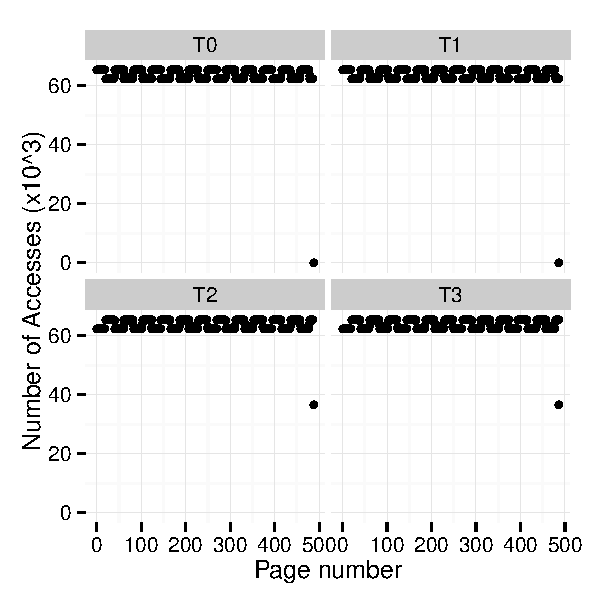
\includegraphics[height=.27\textheight] {mat_B_bloc}
        \label{fig:matrix-B-bloc}
    }
    \subfigure[Structure C (bloc)]{
        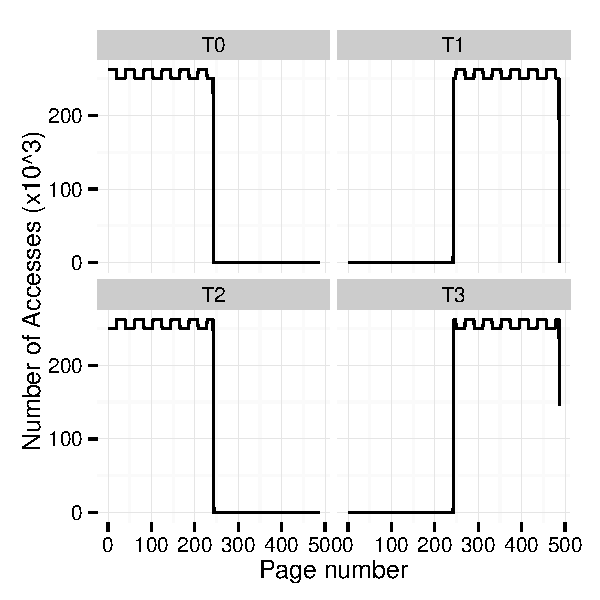
\includegraphics[height=.27\textheight] {mat_C_bloc}
        \label{fig:matrix-C-bloc}
    }
    \caption{By thread access distribution on data structures A and B for the
    bloc matrix multiplication.}
    \label{fig:matrix-bloc}
\end{figure}

As we can see in figure \ref{matrix-bloc}, the bloc algorithm improve the page
locality compared to the naive one. In our algorithm, structures \texttt{B}
and \texttt{C} are not divided the same way, resulting in two different
patterns. For structure \texttt{B} (fig \ref{fig:matrix-B-bloc}), the pages
are interleave, threads $T0$ and $T1$ works on the same pages while threads
$T2$ and $T3$ works on another set of pages. Structures \texttt{B} (and
\texttt{A}, fig \ref{fig:matrix-A-bloc}) are cut in two parts, the first half
is shared by thread $T0$ and $T2$ while the two others works on the second
half. This behaviour provides strong page exclusivity and is therefore more
suitable for NUMA machines. We can easily put each subpart of \texttt{C} (and
\texttt{A}) on a NUMA node and map the thread using it to this node, matrix
\texttt{B} can be distributed using interleave policy.

To test the efficiency of the proposed modification, we compare the execution
time of our modified code (Tabarnac) to the  original code, run without any
improvements (base) and the same code run with full interleave using
\texttt{numactl} (Interleave) and executed with numa balancing enable in the
kernel (Numa Balancing).
\DB{ugly, rewritte needed}

\DB{Todo: use speedup, add interleave}
\begin{figure}[htb]
    \centering
    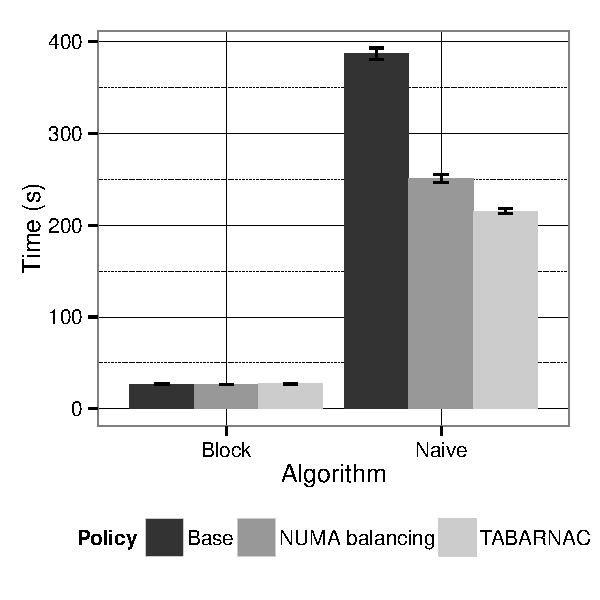
\includegraphics[width=.9\linewidth]{mat_time}
    \caption{Execution time of the matrix multiplication for size $4096*406$ doubles.}
    \label{fig:matrix-res}
\end{figure}

Figure \ref{fig:matrix-res} show the experimental results:

\begin{itemize}
    \item Big improvements for naive: better than every other tools
    \item Not that much for Bloc: algo designed to fit in cache figure
        \ref{fig:matrix-res}
    \item Cncl: \TABARNAC~ will help you modify code to do something like naive
        -> bloc if possible or at least to improve your NUMA mapping as for
        naive.
\end{itemize}


\subsubsection{IS}
\label{sec:exp-is}

\emph{IS} is par of the NAS Parallel benchmarks (OpenMp version)
\cite{Feng04Unstructured}.  It computes an integer sort using a bucket
algorithm. According the NAS parallel benchmark
website\footnote{\url{http://www.nas.nasa.gov/publications/npb.html}, visited
2015-04-25} it has a random memory access. Thus it is a good candidate to be
optimized using \TABARNAC.

\begin{figure}[htb]
    \centering

    \subfigure[\texttt{key\_buff2}]{
        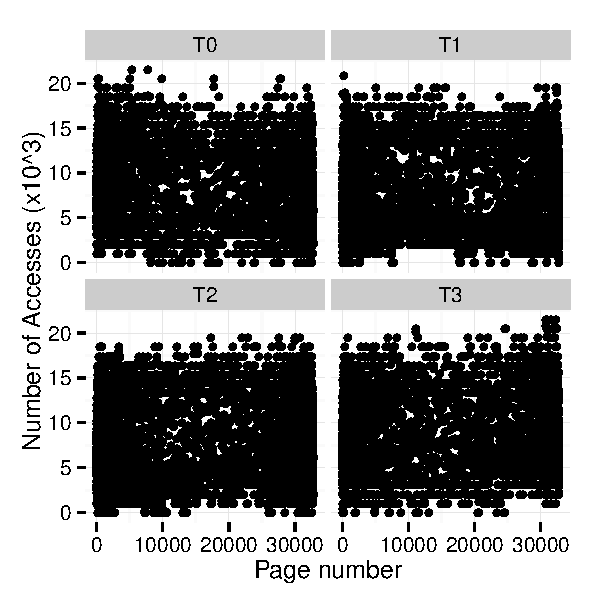
\includegraphics[height=.27\textheight]  {is_w_kb2_orig}
        \label{fig:is-behaviour-orig-kb2}
    }
    \subfigure[\texttt{key\_array}]{
        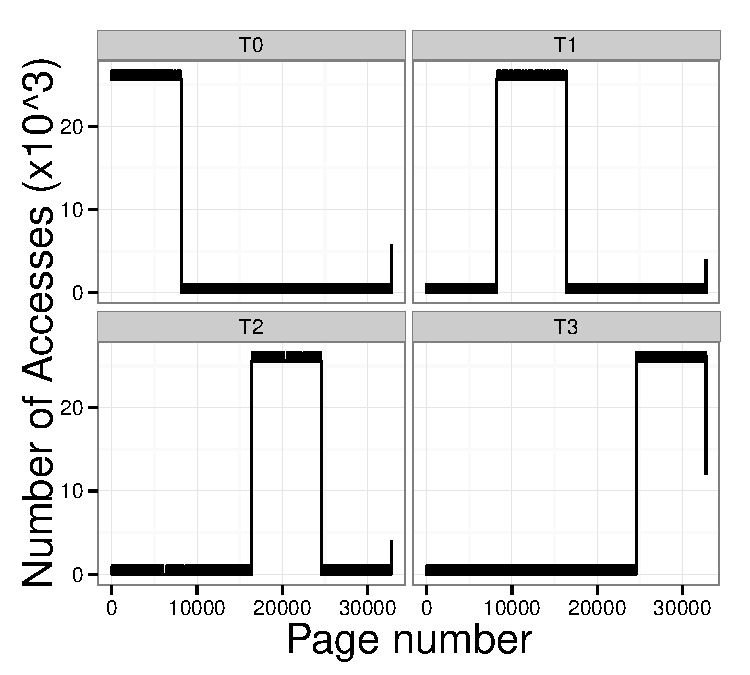
\includegraphics[height=.27\textheight]  {is_w_kba_orig}
        \label{fig:is-behaviour-orig-kba}
    }
    \subfigure[\texttt{key\_buff1}]{
        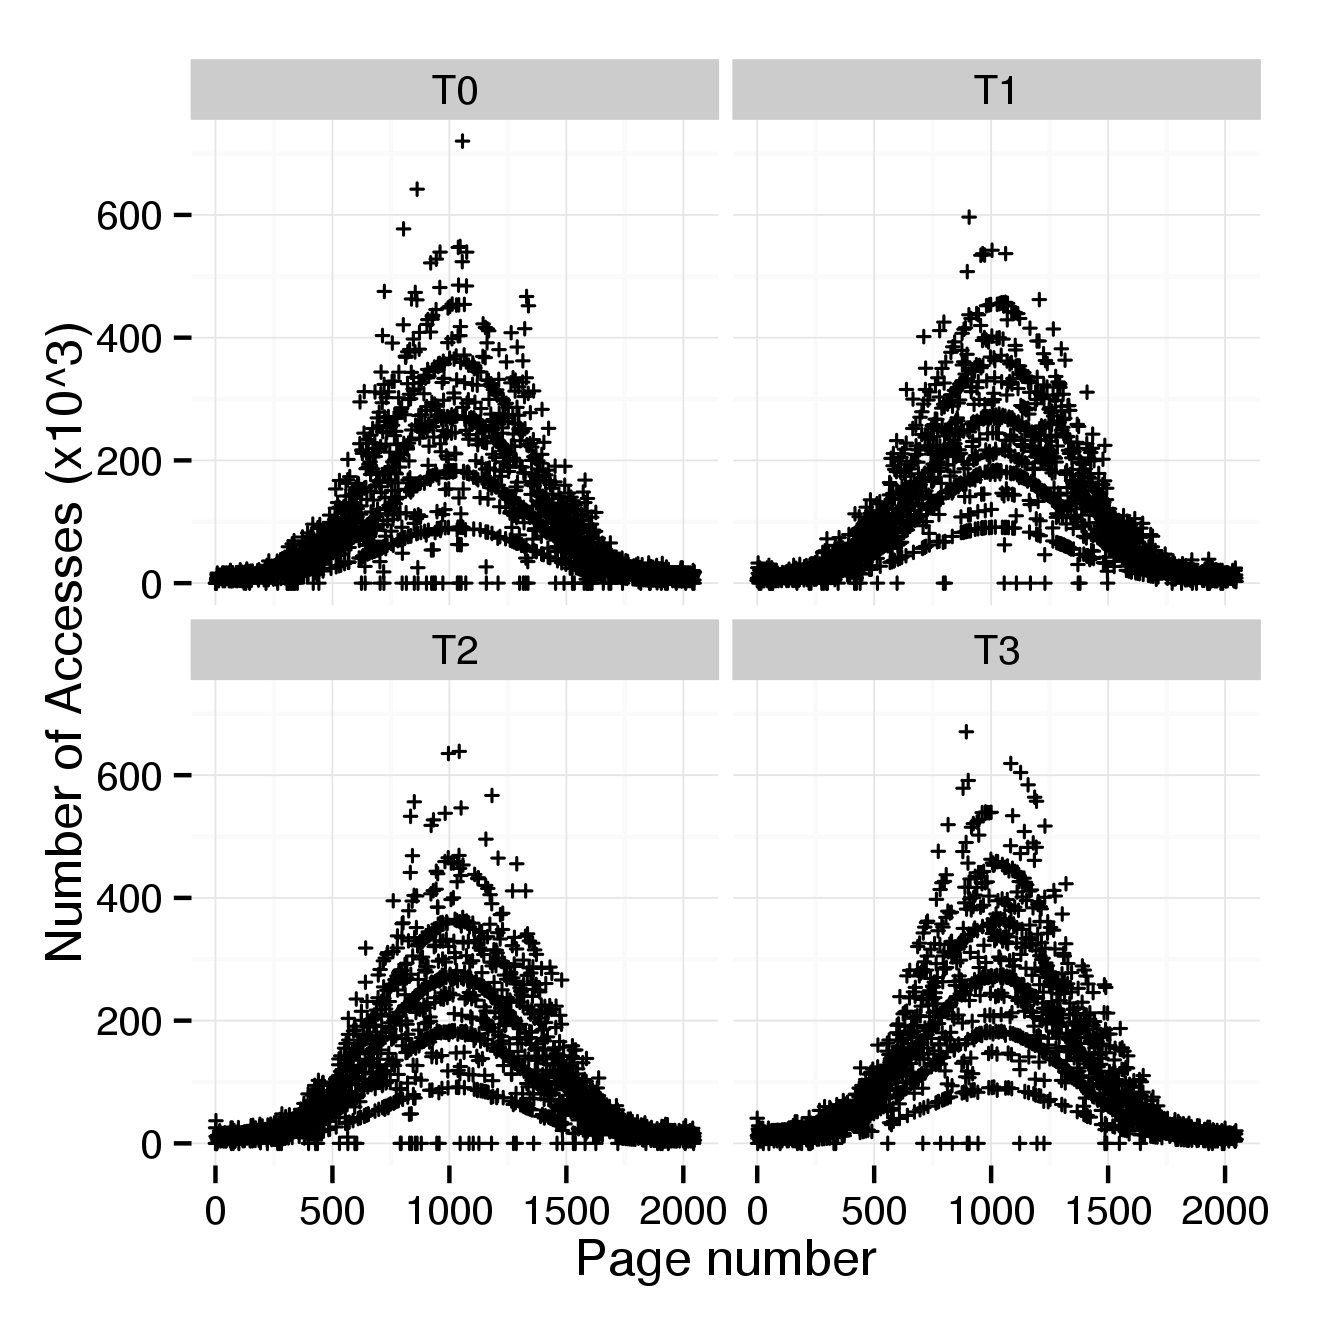
\includegraphics[height=.27\textheight]  {is_w_kb1_orig}
        \label{fig:is-behaviour-orig-kb1}
    }
    \caption{Original memory access distribution for the main structure of
        \emph{IS} with $4$ threads.}
    \label{fig:is-behaviour-orig}
\end{figure}

Figure \ref{fig:is-behaviour-orig} shows the access distributions for the
three main structures of \emph{IS} class W with $4$ threads. We can see that
each of these structures have a different access pattern: \texttt{key\_array}
(fig \ref{fig:is-behaviour-orig-kba}) access distribution shows that every
threads works on a different part of the structures which allows automated
tools to do efficient data/thread mapping on it. However \texttt{key\_buff2}
(fig \ref{fig:is-behaviour-orig-kb2}) is completely shared by every threads,
but the most interesting access distribution is the one of \texttt{key\_buff1}
(fig \ref{fig:is-behaviour-orig-kb1}). Indeed the access repartition seems to
follow a nice Gaussian, which means a few pages are more used than all the
others. With such a distribution, automated tools might generate a lot of page
migration.

\lstinputlisting[caption=\emph{IS} code responsible for the
Gaussian distribution of memory accesses, label=lst:is]{code/is.c}

Using this knowledge, we can look at \emph{IS} code and identify the source of the
Gaussian pattern, indeed all the access to \texttt{key\_buff1} are linear
excepts the one shown in listing \ref{lst:is}\footnote{
    The code has been slightly modified to make it more readable. In the
    original version, the arrays \texttt{key\_buff1} (resp \texttt{key\_buff2})
    are accessed via a generic pointer called \texttt{key\_buff\_ptr} (resp
    \texttt{key\_buff\_ptr2}). More over some comments have been removed as
    they are not necessary here.
}  line \ref{lst:is-gaus}-\ref{lst:is-gaus-end} which depends on the values of
\texttt{key\_buff2}. The comments above the OpenMp loop explains that the
cyclic distribution will result in an unbalanced work distribution. Still we can easily design a cyclic
distribution aware of the Gaussian pattern which provides both a good
distribution of access among the thread and a strong locality. The idea is to
split the loop in two half and give one part of each half to each threads in a
round robin way. We can do that only by modifying line \ref{lst:is-cyclic} as
shown in listing \ref{lst:is-modif}.
\begin{lstlisting}[caption=One line optimization for \emph{IS}, label=lst:is-modif]
#pragma omp for schedule(static,NUM_BUCKETS/(2*omp_get_max_threads()))
\end{lstlisting}

\begin{figure}[htb]
    \centering

    \subfigure[\texttt{key\_buff2}]{
        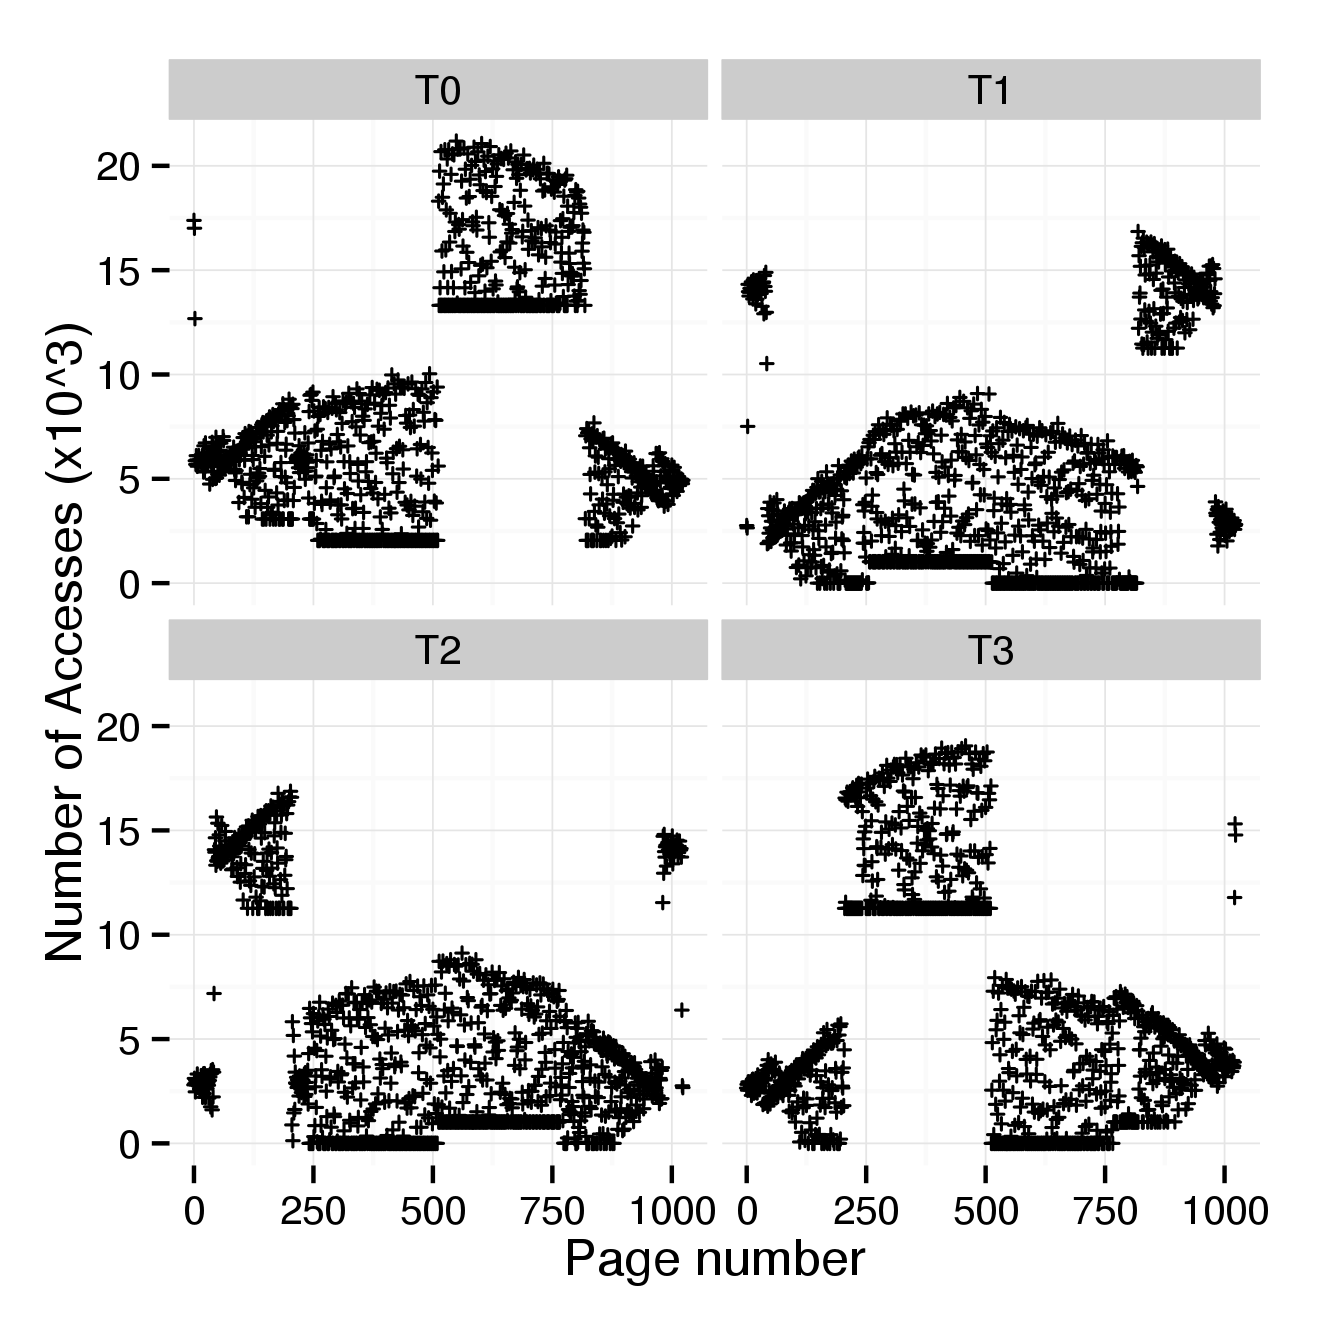
\includegraphics[height=.27\textheight] {is_w_kb2_modif}
        \label{fig:is-behaviour-modif-kb2}
    }
    \subfigure[\texttt{key\_array}]{
        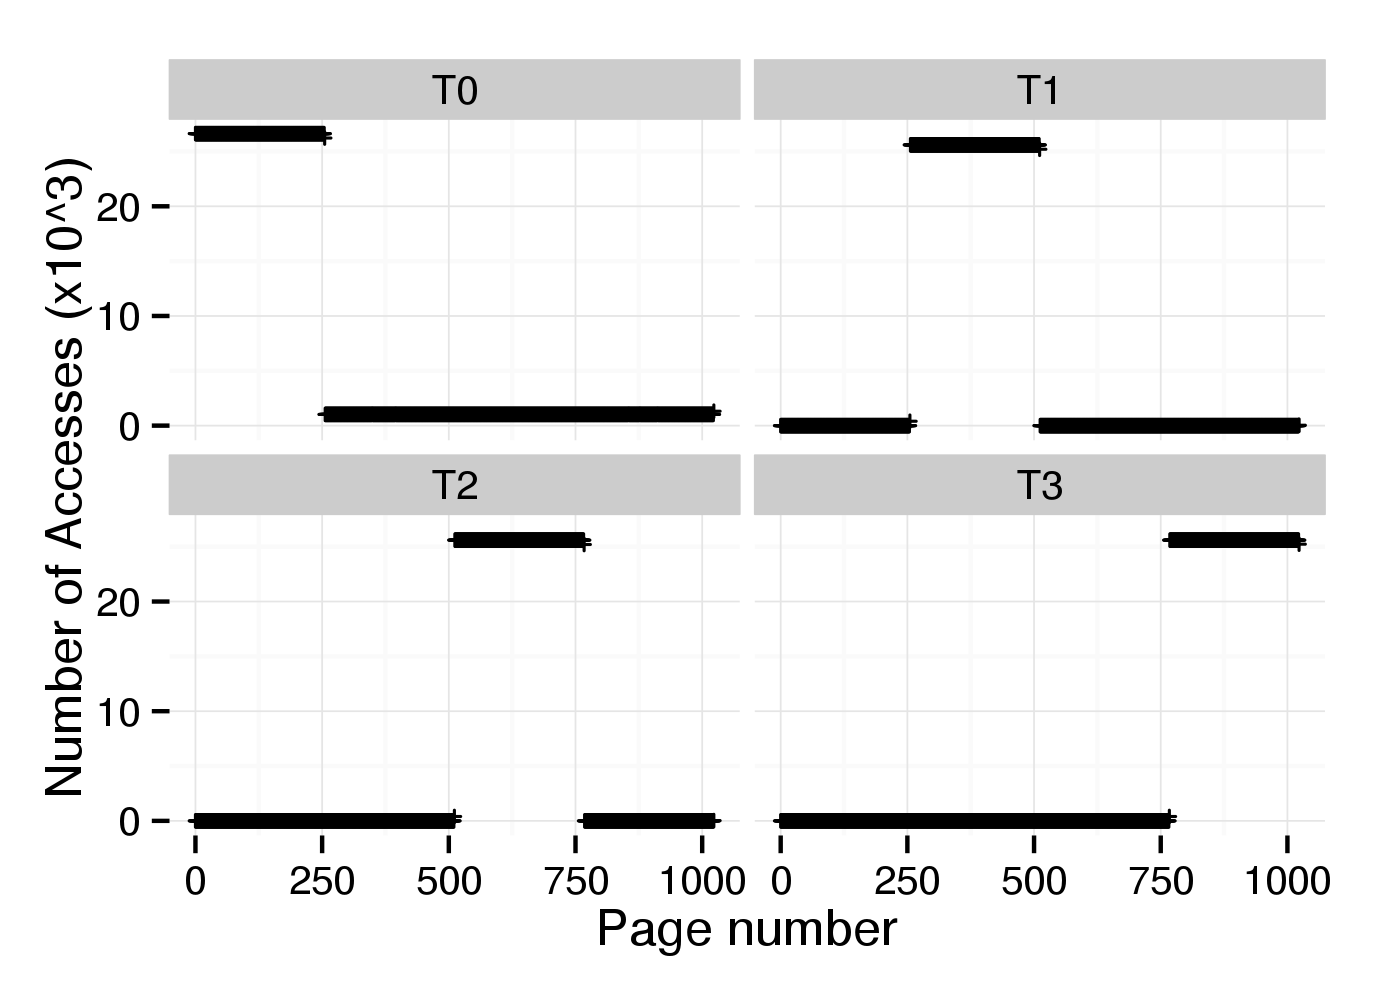
\includegraphics[height=.27\textheight] {is_w_kba_modif}
        \label{fig:is-behaviour-modif-kba}
    }

    \subfigure[\texttt{key\_buff1}]{
        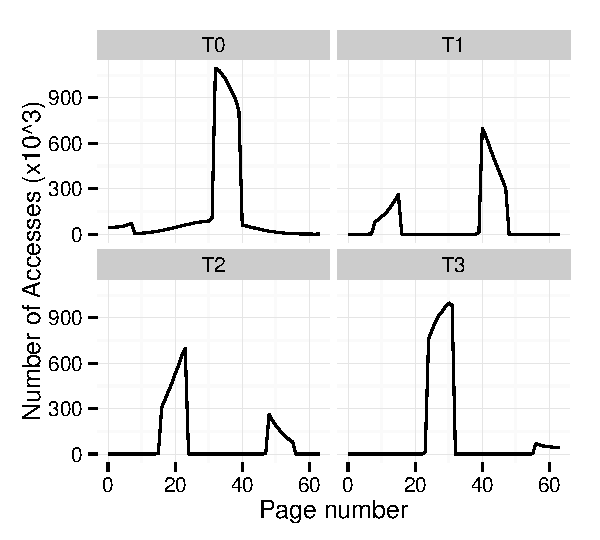
\includegraphics[height=.27\textheight] {is_w_kb1_modif}
        \label{fig:is-behaviour-modif-kb1}
    }
    \caption{Memory access distribution for the main structure of
        \emph{IS} with $4$ threads after our modifications.}
    \label{fig:is-behaviour-modif}
\end{figure}

With this extremely simple code modification we obtain the access distribution
shown in figure \ref{fig:is-behaviour-modif}. We can see that the Gaussian
access of \texttt{key\_buff1} is now distributed over the threads. Each page
of this structure is almost used by only one thread. Moreover
\texttt{key\_buff2} access distribution have also changed, we can see that
each thread uses mostly one part of the array.

The main point of our code modification is to improve the affinity between
thread and memory, therefore we need to pin each thread on a core to keep them
near to their data. To do so we use \texttt{GOMP\_CPU\_AFFINITY}. \TABARNAC~
also shows us that the first touch is always done by the thread actually using
the data for IS, therefore we do not need to map the data on NUMA nodes.
\DB{need to put a plot ?}

We then compare the execution time of \emph{IS.D} for the three scheduling
methods \emph{Dynamic}, \emph{Cyclic} with a step of $1$ and \TABARNAC:
cyclic with the distribution proposed. For the two first methods we compare the
execution time on the bare operation system  (Base), the execution time with
interleave policy (Interleave) and with numa balancing enabled in the kernel
(Numa Balancing). Interleave and Numa Balancing are not relevant with
\TABARNAC~ modifications.

\begin{figure}[htpb]
    \centering
    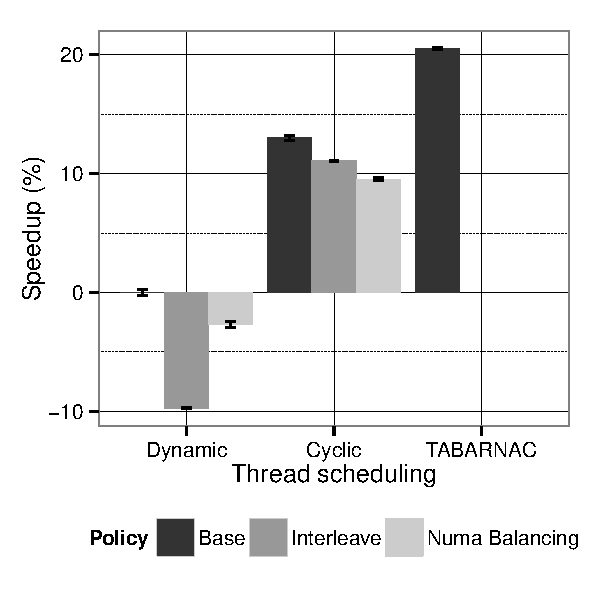
\includegraphics[width=.9\linewidth]{is_exectime.pdf}
    \caption{Speedup for \emph{IS} in class D compared to the default}
\label{fig:is-res}
\end{figure}

Figure\ref{fig:is-res} show the speedup of \emph{IS} in class D compared to
the default version (\emph{dynamic}) for each scheduling method, and for each
optimization technique. The first thing to notice is that with the
\emph{dynamic} scheduling, both Interleave and Numa Balancing slows
the application down. Indeed simple optimization policy are hardly efficient
for non NUMA conscious code.

The cyclic policy, proposed in the original code already provides up to $13\%$
speedup, while the developers clearly explain that it should be slower than
dynamic. We can see that both interleave and Numa Balancing are not suitable 
for this method.

The \TABARNAC~ version provides more than $20\%$ speedup with very small code
modification (two lines of code an \texttt{export} for the thread affinity.
This example shows how analyzing an application's memory behaviour can lead to
significant execution time improvement where automated tools were only slowing
the application down.

\subsubsection{macro-3d}
\label{sec:exp-macro3d}
\DB{Todo mathias}


\begin{figure}[htb]
    \centering

    \subfigure[Access distribution for \texttt{fz}]{
        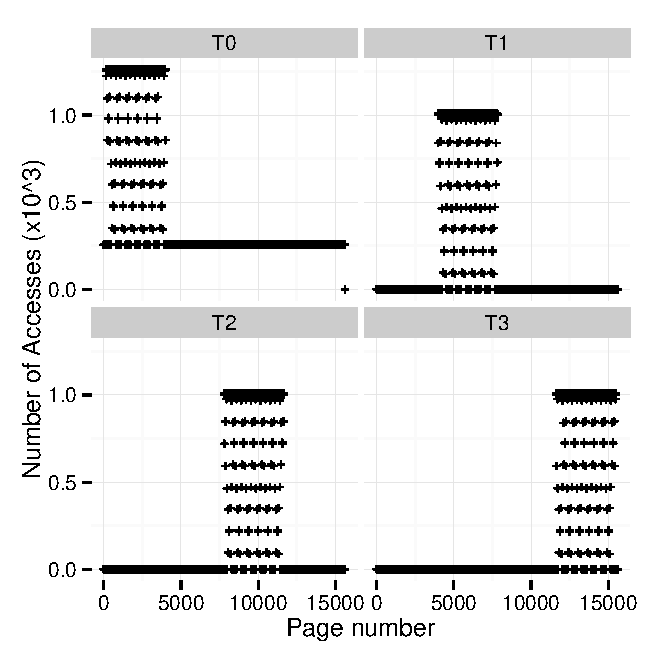
\includegraphics[height=.27\textheight] {macro3d_fz_dist_orig.pdf}
        \label{fig:macro3d-behaviour-fz-orig}
    }
    \subfigure[first touch \texttt{fz}]{
        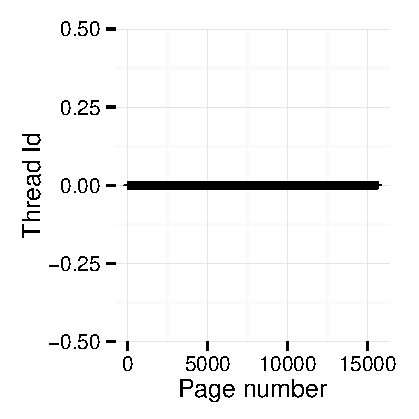
\includegraphics[height=.27\textheight] {macro3d_fz_ft_orig.pdf}
        \label{fig:macro3d-ft-fz-orig}
    }
    \caption{Original access and first touch distribution for \texttt{fz}}
    \label{fig:macro3d-orig}
\end{figure}

\begin{figure}[htb]
    \centering

    \subfigure[Access distribution for \texttt{fz}]{
        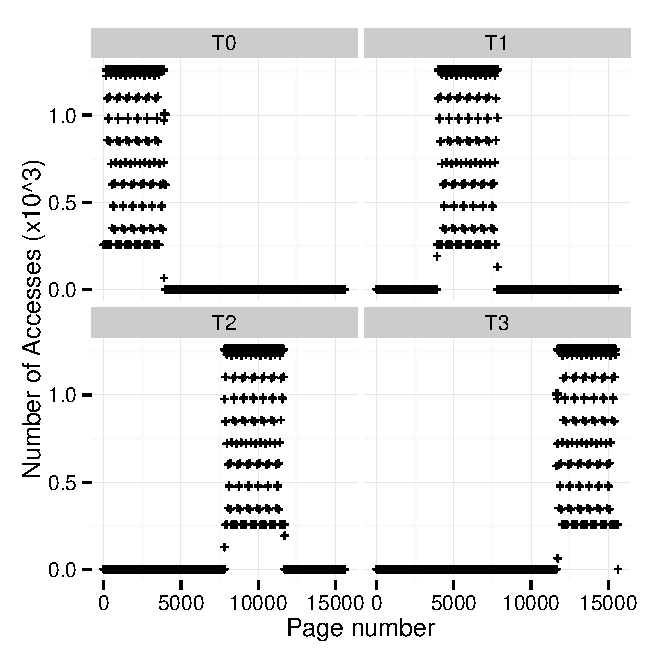
\includegraphics[height=.27\textheight] {macro3d_fz_dist_modif.pdf}
        \label{fig:macro3d-behaviour-fz-modif}
    }
    \subfigure[first touch \texttt{fz}]{
        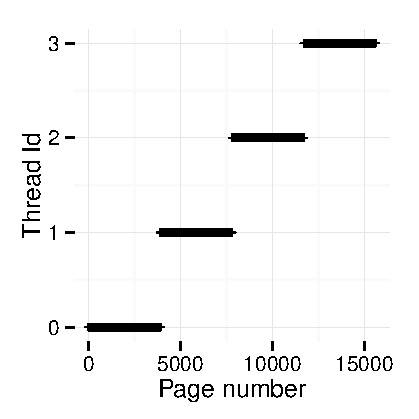
\includegraphics[height=.27\textheight] {macro3d_fz_ft_modif.pdf}
        \label{fig:macro3d-ft-fz-modif}
    }
    \caption{Access and first touch distribution for \texttt{fz} after modifications}
    \label{fig:macro3d-modif}
\end{figure}

\begin{figure}[htpb]
    \centering
    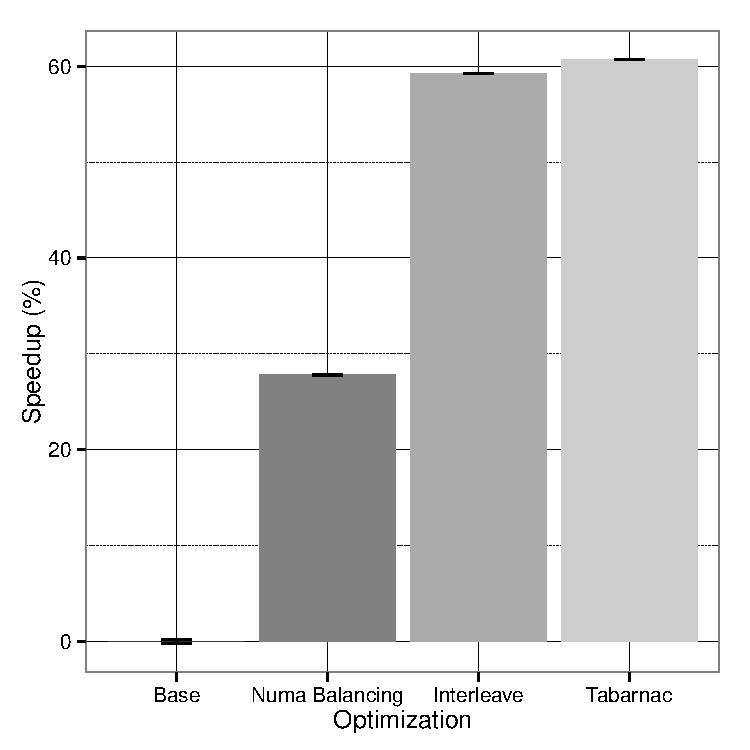
\includegraphics[width=.7\linewidth]{macro3d_exectime.pdf}
    \caption{Speedup for \emph{macro3d} compared to the original application}
\label{fig:is-res}
\end{figure}
